\documentclass{article}

\usepackage[T2A]{fontenc}
\usepackage[a4paper, left=2.5cm, right=1.5cm, top=2.5cm, bottom=2.5cm]{geometry}
\usepackage[russian]{babel}
\usepackage[utf8]{inputenc}
\usepackage{amsfonts}
\usepackage{amsmath}
\usepackage{amssymb}
\usepackage{color}
\usepackage{commath}
\usepackage{graphicx}
\usepackage{hyperref}
\usepackage{mathtools}
\usepackage{parskip}
\usepackage{titling}

\graphicspath{ {./images/} }
\setlength{\droptitle}{-3cm}
\hypersetup{ colorlinks=true, linktoc=all, linkcolor=blue, }

\pagenumbering{arabic}

\begin{document}

  \begin{titlepage}
    \begin{center}
        \vspace*{1cm}
            
        \Huge
        \textbf{Математика 2-й семестр, 10-й класс}
            
        \vspace{5cm}
          
        \Large
        \textbf{Ученики 10-4 класса Оконешников Д.Д. и Паньков М.А. по лекциям Протопоповой Т.В.}
            
        \vfill

        Для внутреннего использования

        \vspace{0.8cm}
        
        \Large
        Россия, г. Новосибирск\\
        СУНЦ НГУ\\
        2021\\
        
            
    \end{center}
  \end{titlepage}
	\newpage
	\tableofcontents
	\thispagestyle{empty}
	\setcounter{tocdepth}{5}
	\newpage
  % \tableofcontents
  % \thispagestyle{empty}
  % \setcounter{tocdepth}{5}
  % \newpage

  \addtocontents{toc}{\protect\contentsline{section}{\protect\numberline{}Элементы теории чисел}{}{}}
  \title{Элементы теории чисел. Теория сравнений.}
  \author{Ученик 10-4 класса Оконешников Д.Д. по лекции к.ф.-м.н. Протопоповой Т.В.}
  \date{от 12 января 2021 г.}
  \maketitle

  \section{Лекция №12}
  
  \textbf{Определение.} \( a \in Z \) и \( b \in Z \backslash \{0\} \) определена операция деления с остатком: разделить целое \( a \) на целое \(b\ (\neq 0) \) с остатком, 
  означает найти такие целые \( q,\ r \in Z \), что \(a=b*q+r,\ 0 \leq r < \abs{b} \).

  \textbf{Определение.} Если при делении с остатком \( r = 0 \), то число \( a \) делится на \( b\ (a \vdots b) \). Число \( b \) при этом называется делителем числа \( a \).

  \textbf{Пример.} \( -7\ \textrm{на}\ 5 \qquad -7 = 5*(-2)+3 \)

  \subsection{Свойства делимости (нацело). ОТА}
  \begin{tabular}{ll}
    \textbf{(1)} Если \( a \vdots c \) и \(b \vdots c\), то \( (a \pm b) \vdots c \) & \textbf{(5)} \( a \vdots b \) и \( b \vdots a \Rightarrow \abs{a} = \abs{b} \)\\
    \( \uparrow
      \begin{aligned}
        &a = cq_1\\
        &b = cq_2
      \end{aligned}
    \Rightarrow (a \pm b) = c(q_1 \pm q_2) \Rightarrow (a \pm b) \vdots c \downarrow \) & \textbf{(6)} \( \forall\ a \in Z \backslash \{0\} \Rightarrow 0 \vdots a \)\\
    \textbf{(2)} \( a \vdots b \Rightarrow ak \vdots b\ (k \in Z)\) & \textbf{(7)} \( \forall\ a \in Z \Rightarrow a \vdots 1 \)\\
    \textbf{(3)} \( a \vdots b,\ b \vdots c \Rightarrow a \vdots c \) & \textbf{(8)} Если \( ab \vdots m \) и \( \textrm{НОД}(a,\ m) = 1, \textrm{ то } b \vdots m \)\\
    \( \uparrow a = bq_1,\ b=cq_2 \Rightarrow a = c*(q_1*q_2) \Rightarrow a \vdots c \downarrow \) & \textbf{(9)} Если \(a \vdots m,\ a \vdots k \textrm{ и НОД}(m,\ k) = 1, \textrm{ то } a \vdots mk \)\\
    \textbf{(4)} Если \( a \neq 0,\ a \vdots b \Rightarrow \abs{a} \geq \abs{b} \) &\\
    \( \uparrow a \vdots b \Leftrightarrow a = b*q \Rightarrow \abs{a} = \abs{b} * \abs{q} \Rightarrow \) от противного, &\\
    если \( \abs{a} < \abs{b} \), то \( \abs{q} = \frac{\abs{a}}{\abs{b}} < \frac{\abs{b}}{\abs{b}} = 1 \Rightarrow \) единственная &\\
    возможность при целом \( q = 0 \), но тогда и \( a = 0 \).&\\
    Противоречие. \( \downarrow \) &\\
  \end{tabular}

  \textbf{Определение.} Натуральное число \( p > 1 \) называется простым, если оно имеет ровно два натуральных делителя \( (p \textrm{ и } 1) \).

  
  Все остальные натуральные числа называются составными (кроме 1). Единица не является ни простым, ни составным.
  
  \subsubsection{Основная теорема арифметики}
  \textbf{Th.1} (Основная теорема арифметики) Всякое натуральное число \( n > 1 \) может быть представлено в виде \( n = p_1*p_2* ... *p_i \), где \( p_i \) --- простые числа. Это представление единственно с точностью до порядка множителей (т.е. если \( n = p_1*p_2*...*p_r = q_1*q_2*...*q_s \), то \( r = s \) и \(q_1,\ q_2,...,\ q_s \) можно перестановкой получить из чисел \( p_1,\ p_2,...,\ p_r \))

  \textbf{(1)} \underline{Докажем существование} 

  Пусть \(n \in \mathbb{N},\ n > 1 \). Среди делителей \( n \) есть числа превосходящие 1 (например, само \( n \)). Пусть \( p_1 \) --- наименьший из таких делителей.

  \( p_1 \) --- простое число (если оно само имело бы делитель \( 1 < a < p_1 \), то \( a \) было бы меньше \( p_1 \) и было бы делителем \( n \) (св-ва 4,3), противоречит тому, что выбран наименьший делитель).

  Итак, \( n = p_1n_1, \textrm{ где } p_1 \textrm{ --- простое, } n_1 \in \mathbb{N} \textrm{ и } n_1 < n \) (св-во 4).

  Если \( n_1 > 1 \), то поступим с ним так же, как и числом \( n \), представим его в виде \( n_1 = p_2n_2 \), \( p_2 \) --- простое, \( n_2 \in \mathbb{N}, n_2 < n_1 \Rightarrow n = p_1*p_2*n_2 \) и т.д.

  В конце концов, так как \( n_i \in \mathbb{N}, i=1,2,3,... \) убывают, то \( \exists\ n_r = 1 \) и процесс обрывается: \( n=p_1*p_2*...p_r \)

  \textbf{(2)} \underline{Докажем существование (единственность)}
  От противного. Если \( \exists \) хоть одно натуральное число, допускающее два существенно различных разложения, то непременно \( \exists \) и \underline{наименьшее} число с таким свойством: \[ m = p_1*p_2*...*p_r = q_1*q_2*...*q_s \qquad (1) \]
  Можем допустить, что \( p_1 \leq p_2 \leq ... \leq p_r; q_1 \leq q_2 \leq ... \leq q_s \).

  А) Заметим, что \( p_1 \neq q_1 \).\\
  Если равны, то разделив (1) на \( p_1 = q_1 \), получили бы два существенно различных разложения на простые множители для числа \( < m \) (Противоречие с тем, что \( m \) --- наименьшее).\\
  На самом деле показали больше: что среди \( q_j \) нет чисел равных какому-либо \( p_i \)

  Б) Из А) \( p_1 < q_1 \) или \( p_1 > q_1 \). Пусть \( p_1 < q_1 \) (для \( p_1 > q_1 \) доказательство строится аналогично).\\
  Рассмотрим целое число: \[ m' = m - p_1*q_2*...*q_s\qquad (2) \]
  Подставляя вместо \( m \) два его разложения, получим: \[ m' = p_1*p_2*...*p_r - p_1*q_2*...*q_s = p_1(p_2*...*p_r - q_2*...*q_s)\qquad (3) \] \[ m' = q_1*q_2*...*q_s - p_1*q_2*...*q_s = (q_1 - p_1)q_2*...*q_s\qquad (4) \]
  Из равенства (4) очевидно \( m' > 0 \). Из равенства (2) \( m' < m \), а значит, для \( m' \) разложение на простые множители --- единственно (с точностью до порядка сомножителей).

  Из (3) \( \Rightarrow p_1 \) входит множителем в \( m' \), значит, из (4) \( p_1 \) входит множителем либо в \( q_1 - p_1 \), либо в \( q_2*...*q_s \). Но последнее невозможно, так как все \( q_j > p_1\ (p_1 < q_1) \) и они простые.
  
  Значит, \( p_1 \) входит множителем в \( q_1 - p_1 \), т.е. \( \mathbf{(q_1 - p_1) \vdots p_1} \) \( \Rightarrow q_1 - p_1 = p_1h \Rightarrow q_1 = p_1(h + 1) \), т.е. \( \mathbf{q_1 \vdots p_1} \), чего быть не может. Противоречие. Ч.Т.Д.

  \subsubsection{Теорема Евклида}
  \textbf{Th.2} (Теорема Евклида) Множество простых чисел бесконечно.

  \( \uparrow \) Доказательство проведем от противного. Предположим, что множество простых чисел конечно, т.е. \( P=\{p_1,p_2,...p_k\} \) --- конечная совокупность простых чисел.

  Рассмотрим число \( p = p_1*p_2*...*p_k + 1 \).

  Заметим, что \( \forall\ i, i=1,2,...,k \) это \( p > p_i \), т.е. \( p \notin P \), значит, оно составное и по ОТА может быть представлено в виде произведения простых множителей.

  Но \( p \) не делится ни на какой \( p_i \) (при делении дает в остатке 1).

  Значит, наше предположение о конечности системы простых чисел неверно. \( \downarrow \)

  \textbf{Утверждение.} Существуют сколь угодно длинные участки натурального ряда, вовсе не содержащие простых чисел

  \( \uparrow \) Действительно, пусть \( n \in \mathbb{N}, n > 1 \). Рассмотрим ряд чисел: \( n! + 2,n! + 3,...,n! + n \).
  
  \begin{tabular}{ll}
    \( n = 2: 2! + 2 \) --- одно число в ряду; &\\
    \( n = 3: 3! + 2, 3! + 3 \) --- два числа в ряду; & чем больше \( n \), тем больше в ряду\\
    \( n = 4: 4! + 2, 4! + 3, 4! + 4 \) --- три числа в ряду; & чисел (\( n - 1 \) число).\\
    и т.д. &\\
  \end{tabular}

  В этом ряду нет ни одного простого числа, так как \( n! + 2 \) делится на 2, \( n! + 3 \) делится на 3, \( n! + n \) делится на n. Таким образом, при больших \( n \) такие участки натурального ряда могут быть очень большими. \( \downarrow \) 

  \subsection{Каноническое разложение числа. НОД. НОК}
  \subsubsection{Теорема Эйлера}
  \textbf{Th.3} (Теорема Эйлера) Пусть \( \tau(n) \) --- количество простых чисел \( \leq n \). Тогда \[ \frac{\tau(n)}{n} \xrightarrow[n \rightarrow \infty]{} 0 \]
  Понятно, что \( \tau(n) \) увеличивается (т.е. \( \rightarrow \infty \)) при \( n \rightarrow \infty \) (это означает, что простые числа встречаются все реже и реже).

  Мы показали, что любое натуральное число мы можем представить в виде произведения простых множителей (и такое представление единственно с точностью до перестановки множителей): \( n = p_1*p_2*...*p_r,\ p_1 \leq p_2 \leq ... \leq p_r \). Используя обозначение степени, можем записать так: \[ \mathbf{n = p_1^{a_1}*p_2^{a_2}*...*p_k^{a_k}}, \textrm{ (каноническое разложение) } \] 
  \[ \textrm{где } p_1 < p_2 < ... < p_k \textrm{ --- простые, } a_1, a_2, ..., a_k \textrm{ --- натуральные числа.} \]
  \textit{Замечание.} Бывает полезно записать в разложение \underline{все} простые числа \( \leq p_k \) и использовать показатель равный 0.

  Если число \( m \) является делителем \( n \), то несложно понять, что \( \mathbf{m = p_1^{\beta_1}*p_2^{\beta_2}*...*p_k^{\beta_k}} \), где \( 0 \leq \beta_i \leq a_i \).

  Можно посчитать число всех натуральных делителей числа \( n \). Любой делитель \( n \) имеет следующую структуру: \( \mathbf{m = p_1^{0,1,2,...,a_1}*p_2^{0,1,...a_2}*...*p_k^{0,1,...,a_k}} \)

  Для первого множителя \( (a_1 + 1) \) возможность для второго \( (a_2 + 1) \) возможностей и т.д. Таким образом, число всех делителей \( (a_1 + 1)*(a_2 + 1)*...*(a_k + 1) \).

  \textbf{Пример.} Сколько делителей у числа 120 (включая 1 и само число)?

  \begin{tabular}{r|l}
    120 & 2\\
    60 & 2\\
    30 & 2\\
    15 & 3\\
    5 & 5\\
    1 & \\
  \end{tabular}

  \( 120 = 2^3 * 3^1 * 5^1 \). Значит, число всех делителей \( = (3 + 1)*(1 + 1)*(1 + 1) = 4*2*2 = 16 \).

  \textbf{Определение.} \( d \) --- общий делитель \( a \) и \( b \Leftrightarrow \mathbf{a \vdots d } \) и \( \mathbf{b \vdots d} \).

  \textbf{Определение.} Наибольший общий делитель чисел \( a \) и \( b \) обозначается \( \textrm{НОД}(a, b) \).

  \textbf{Определение.} Наименьшее общее кратное \( \textrm{НОК}(a, b) = k \) --- наименьшее натуральное число такое, что \( \mathbf{k \vdots a} \) и \( \mathbf{k \vdots b} \).

  Пусть \( \mathbf{a = p_1^{a_1} * p_2^{a_2} * ... * p_k^{a_k}},\ \mathbf{b = p_1^{\beta_1} * p_2^{\beta_2} * ... * p_k^{\beta_k}} \)

  Здесь использовали показатель 0 для тех простых множителей, которые входят только в одно из разложений.

  Тогда \[ \textrm{НОД}(a, b) = p_1^{min(a_1, \beta_1)} * p_2^{min(a_2, \beta_2)} * ... * p_k^{min(a_k, \beta_k)} \]
  \[ \textrm{НОК}(a, b) = p_1^{max(a_1, \beta_1)} * p_2^{max(a_2, \beta_2)} * ... * p_k^{max(a_k, \beta_k)} \]
  \[ \textrm{НОД}(a, b)*\textrm{НОК}(a, b) = a * b \]

  \textbf{Пример.} \( a = 2 * 3^3 * 5^2 * 7,\ b = 2^2 * 3 * 7^2 * 11 \Rightarrow a = 2^1 * 3^3 * 5^2 * 7^1 * 11^0,\ b = 2^2 * 3^1 * 5^0 * 7^2 * 11^1 \Rightarrow \textrm{НОД}(a, b) = 2^1 * 3^1 * 5^0 * 7^1 * 11^0,\ \textrm{НОК}(a, b) = 2^2 * 3^3 * 5^2 * 7^2 * 11^1 \).

  Чтобы получить каноническое разложение полезно помнить признаки делимости.
  
  1) на 2 и 5. Легко.\\
  2) на 4. \( n = \overline{a_ka_{k-1}...a_1a_0} = 100 * \overline{a_ka_{k-1}...a_2} + \overline{a_1a_0}.\quad 100 \vdots 4.\ \Rightarrow n \vdots 4 \Leftrightarrow \overline{a_1a_0} \vdots 4 \).\\
  3) на 8. \( n \vdots 8 \Leftrightarrow \overline{a_2a_1a_0} \vdots 8 \).\\
  4) на 3. \( n = \overline{a_ka_{k-1}...a_1a_0} = a_k10^k + a_{k-1}10^{k-1} + ... + a_1 10 + a_0 = a_k(\underbrace{999...9}_k + 1) + a_{k-1}(\underbrace{999...9}_{k-1} + 1) + ... + a_1(9 + 1) + a_0 = (a_k\underbrace{999...9}_k + a_{k-1}\underbrace{999...9}_{k-1} + ... + a_1 9) + (a_k + a_{k-1} + ... + a_1 + a_0) \)\\
  Аналогично для 9.\\
  5) на 6. \( n \vdots 2 \) и \( n \vdots 3 \Rightarrow \) (так как 2 и 3 взаимно просты) \( n \vdots 6 \)\\
  6) на 11. \[ n = \overline{a_ka_{k-1}...a_1a_0} = a_0 + a_1 10 + a_2 100 + a_3 + 1000 + ... + a_k 10^k = \] 
  \[ = a_0 + a_1(11 - 1) + a_2(99 + 1) + a_3(1001 - 1) + a_4(9999 + 1) + a_5(100001 - 1) + ... + a_k 10^k = \] 
  \[ = (a_0 - a_1 + a_2 - a_3 + a_4 - ...) + (a_1 11 + a_3 1001 + a_5 100001 + ... + a_{2l+1}1\underbrace{00...0}1_{2l} + ... ) +\]
  \[ + (a_2 99 + a_4 9999 + ... + a_{2m}\underbrace{99...99}_{2m} + ...)\]\\
  А) числа, состоящие из четного числа 9-ок, делятся на 11, т.е. последняя скобка \( \vdots 11 \);\\
  Б) заметим, что \( 1001 = (1100 - 99) \vdots 11,\quad 100001 = (110000 - 9999) \vdots 11,\quad 1\underbrace{00...00}_{2l}1 = (11\underbrace{00...00}_{2l} - \underbrace{99...99}_{2l} \vdots 11) \).

  \subsubsection{Алгоритм Евклида нахождения НОД(a,b)}
  Пусть требуется найти НОД\( (a,b) \). Будем считать, что \( \abs{a} > \abs{b} \).

  \textbf{1)} Разделим \( a \) на \( b \) с остатком: \[ a = q_1b + r_1,\ 0 \leq r_1 < \abs{b}\quad (1) \]
  Заметим, что любой делитель пары \( a \) и \( b \) будет делителем \( r_1 \), а значит пары \( b \) и \( r_1 \). С другой стороны, любой делитель пары \( (b,r_1) \) будет делителем \( a \), а значит пары \( (a,b) \). Таким образом (равенство множеств), множество делителей пары \( (a,b) \) совпадает с множеством делителей пары \( (b,r_1) \), а значит и НОД\( (a,b) \) = НОД\( (b,r_1) \).

  \textbf{2)} Разделим \( b \) на \( r_1 \) с остатком: \[ b = q_2r_1 + r_2,\ 0 \leq r_2 < r_1\quad (2) \]
  При этом получаем, что НОД\( (b,r_1) \) = НОД\( (r_1,r_2) \)

  \textbf{3)} Разделим \( r_1 \) на \( r_2 \) с остатком: \[ r_1 = q_3r_2 + r_3,\ 0 \leq r_3 < r_2\quad (3) \]
  При этом НОД\( (r_1, r_2) \) = НОД\( (r_2, r_3) \).\\
  И т.д.

  Посмотрим на остатки. \( \abs{b} > r_1 > r_2 > r_3 > ... \geq 0 \). Получили строго убывающую последовательность неотрицательных целых чисел. Эта последовательность конечна. Существует \( r_{k+1} = 0 \), т.е.

  \textbf{k+1)} \[ r_{k-1} = q_{k+1}r_k + 0\quad (k+1) \]
  При этом НОД\( (a,b) \) = НОД\( (b,r_1) \) = НОД\( (r_1,r_2) \) = НОД\( (r_2,r_3) \) = ... = НОД\( (r_{k-1},r_k) = r_k \).\\
  Таким образом, НОД\( (a,b) \) равен последнему ненулевому остатку в алгоритме Евклида.

  \begin{tabular}{ll}
    Весь алгоритм: & \textbf{Пример.} НОД(5083,3553)-?\\
    \textbf{1)} \( a = q_1b + r_1,\ 0 \leq r_1 < \abs{b} \) & \( 5083 = 1*3553 + 1530 \)\\
    \textbf{2)} \( b = q_2r_1 + r_2,\ 0 \leq r_2 < \abs{r_1} \) & \( 3553 = 2*1530 + 493 \)\\
    \textbf{3)} \( r_1 = q_3r_2 + r_3,\ 0 \leq r_3 < \abs{r_2} \) & \( 493 = 9*51 + 34 \)\\
    ...& \( 51 = 1*34 + 17 \)\\
    \textbf{k)} \( r_{k-2} = q_kr_{k-1} + r_k \) & \( 34 = 2*17 + 0 \Rightarrow \textrm{НОД}(5083,3553) = 17\)\\
    \textbf{k+1)} \( r_{k-1} = q_{k+1}r_{k} + 0 \) & \\
    \( \textrm{НОД}(a,b) = r_k \) & \\
  \end{tabular}
  
    % \tableofcontents
    % \thispagestyle{empty}
    % \setcounter{tocdepth}{5}
    % \newpage

    % \addtocontents{toc}{\protect\contentsline{section}{\protect\numberline{}Элементы теории чисел}{}{}}
    \title{Элементы теории чисел. Теория сравнений.}
    \author{Ученик 10-4 класса Оконешников Д.Д. по лекции к.ф.-м.н. Протопоповой Т.В.}
    \date{от 20 января 2021 г.}
    \maketitle

    \section{Лекция №13}
    \subsection{Каноническое разложение числа. НОД. НОК}
    
    \begin{tabular}{ll}
        Весь алгоритм: & \textbf{Пример.} НОД(5083,3553)-?\\
        \textbf{1)} \( a = q_1b + r_1 \) & \( \Rightarrow r_1 = a - q_1b = A_1a + B_1b \)\\
        \textbf{2)} \( b = q_2r_1 + r_2 \) & \( \Rightarrow r_2 = b - q_2r_1 = b - q_2(A_1a + B_1b) = -q_2A_1a + (1 - B_1q_2)b = A_2a + B_2b \)\\
        \textbf{3)} \( r_1 = q_3r_2 + r_3 \) & \( \Rightarrow r_3 = r_1 - q_3r_2 = A_1a + B_1b - q_3(A_2a + B_2b) =  \)\\
        ...& \( = (A_1 - q_3A_2)a + (B_1 - q_3B_2)b = A_3a + B_3b \)\\
        \textbf{k)} \( r_{k-2} = q_kr_{k-1} + r_k \) & \( r_k = A_ka + B_kb \textrm{ или НОД}(a,b)=Aa + Bb \), где \( A,\ B \) --- целые\\
        \textbf{k+1)} \( r_{k-1} = q_{k+1}r_{k} + 0 \) & \\
        \( \textrm{НОД}(a,b) = r_k \) & \\
    \end{tabular}

    \textbf{Утверждение.} Если \( d = \textrm{ НОД}(a,b) \), то существуют целые \( A \) и \( B: d = Aa + Bb \).

    \textbf{Замечание.} Если \( \textrm{НОД}(a,b) = 1 \) (т.е. \( a \) и \( b \) взаимно просты), то существуют целые \( A \) и \( B: 1 = Aa + Bb \).

    \subsection{Доказательство свойств делимости 8 и 9}
    \textbf{Свойство 8.} Если \( ab \vdots m \) и \( \textrm{НОД}(a, m) = 1 \), то \( b \vdots m \)

    \( \uparrow \) Имеем \( \textrm{НОД}(a,m) = 1 \Rightarrow \exists A,\ M: Aa + Mm = 1. \)\\
    Домножим последнее равенство на \( b: \underset{\vdots m}{Aab} + \underset{\vdots m}{Mmb} = b \Rightarrow b \vdots m \downarrow \)

    \textbf{Свойство 9.} Если \( a \vdots m,\ a \vdots k \) и \( \textrm{НОД}(m,k) = 1 \), то \(a \vdots mk \)

    \( \uparrow \)

    1) \( a \vdots m \Rightarrow a = mq_1 \)\\
    2) \( a \vdots k \Rightarrow mq_1 \vdots k \)\\
    3) из 2) и \( \textrm{НОД}(m,k) = 1 \Rightarrow \) по свойству 8 \( q_1 \vdots k \Rightarrow q_1 = kq_2 \)\\
    4) \( a = mq_1 = mkq_2 \), т.е. \( a \vdots mk \downarrow \)

    \subsection{Решение уравнений ax + by = c}
    \textbf{Определение.} Диофантово уравнение первой степени - уравнение вида \( ax + by = c \), где \( a,b,c,x,y \) --- целые числа.

    Пусть \( \textrm{НОД}(a,b) = d \).

    1) Если \( c \vdots d \), то делим на \( d \) правую и левую части уравнения и получаем \( a_1x + b_1y = c_1 \), где \( \textrm{НОД}(a_1, b_1) = 1 \).\\
    2) Если \( c \) не делится на \( d \), то уравнение решений не имеет.\\

    Таким образом, будем рассматривать уравнения (*) \( ax + by = c,\ \textrm{НОД}(a,b) = 1 \).
    
    Так как \( \textrm{НОД}(a, b) = 1 \), то по следствию из алгоритма Евклида \( \exists \) целые \( A,\ B: Aa + Bb = 1 \).\\
    Домножим равенство на \( c: Aca + Bcb = c \).\\
    Видим, что пара целых чисел \( (x_0,y_0) = (Ac, bc) \) является решением уравнения.\\
    Мы нашли частное (одно из) решение нашего уравнения. Найдем все решения \( (x,y) \).\\

    \[ \begin{cases}
        ax_0 + by_0 = c,\\
        ax + by = c.
    \end{cases} \Rightarrow a(x - x_0) + b(y - y_0) = 0,\ a(x - x_0) = -b(y - y_0) \]
    \( \textrm{НОД}(a,b) = 1 \), значит \( (x - x_0) \vdots b \), т.е. \( x - x_0 = bt \) или \( x = x_0 + bt \), где \( t \) --- целое.\\
    Тогда \( y - y_0 = \frac{-a(x - x_0)}{b} = -at \) или \( y = y_0 - at \).\\
    Таким образом, все пары вида \( (x_0 + bt, y_0 - at) \), где \( t \) --- целое, являются решениями (*).

    \textbf{Замечание.} Общее решение диофантова уравнения представляет собой сумму частного решения уравнения и решения соответствующего однородного уравнения (уравнения \( ax + by = 0 \)).

    Легко понять, что решениями однородного уравнения являются все пары вида \( (bt, -at) \), где \( t \) --- целое.

    \textbf{Пример.} 7x - 23y = 131
    Проверка решения: \( c\ \vdots \ \textrm{НОД}(a,b) \Rightarrow \) имеет решения.\\ 
    Можно угадать частное решение (22,1), так как 154 - 23 = 131.\\
    Тогда все решения --- \( (22-33t,1-7t) \), \( t \in \mathbb{Z} \).

    \addtocontents{toc}{\protect\contentsline{section}{\protect\numberline{}Теория сравнений}{}{}}
    \subsection{Сравнения}

    Основная идея теории сравнений заключается в том, что два числа \( a \) и \( b (\in \mathbb{Z}) \), имеющие при делении на \( m \in \mathbb{N} \) один и тот же остаток, обнаруживают целый ряд одинаковых свойств по отношению к \( m \).

    Так по отношению к 2 мы выделяем четные и нечетные числа. Знаем, например, что сумма/разность четных - четное число, произведение четных - четное и т.д.

    \textbf{Определение.} Целые числа \( a \) и \( b \) называются сравнимыми по модулю \( m (a \equiv b (mod\ m)) \), если при делении на \( m \) они дают одинаковые остатки. \textbf{(1)}
    
    \textbf{Пример.} \( 8 \equiv 3 (mod\ 5) \equiv 103 (mod\ 5) \equiv -2 (mod\ 5) \equiv -17 (mod\ 5) \) и т.д.

    \textbf{Определение.} \( a \equiv b (mod\ m) \Leftrightarrow (a - b) \vdots m \). \textbf{(2)}

    Докажем эквивалентность определений 1 и 2.\\
    \( \uparrow \)\\
    1) \textbf{(1)} \( \Rightarrow \) \textbf{(2)}. Пусть остатки одинаковы, т.е. \( a = q_1m + r,\ b = q_2m + r \Rightarrow a - b = m(q_1 - q_2),\ (q_1 - q_2) \in \mathbb{Z} \), т.е. \( (a - b) \vdots m \);\\
    2) \textbf{(2)} \( \Rightarrow \) \textbf{(1)}. От противного.\\
    Пусть остатки разные, т.е. \( a = q_1m + r_1,\ b = q_2m + r_2 \), где \( 0 \leq r_1 < \abs{m},\ 0 \leq r_2 < \abs{m} (-\abs{m} < -r_2 \leq 0) \).\\
    Тогда \( a - b = m(q_1 - q_2) + r_1 - r_2 \) и \( -\abs{m} < r_1 - r_2 < \abs{m} (\abs{r_1 - r_2} < \abs{m} \mathbf{(3)}) \Rightarrow (r_1 - r_2) \vdots m \)\\
    Но тогда по свойству делимости 4, если \( r_1 - r_2 \neq 0 \), то \( \abs{r_1 - r_2} \geq \abs{m} \), противоречие с \textbf{(3)}. Таким образом, \(r_1 = r_2. \downarrow \)

    \subsection{Свойства сравнений}
    1) \( a \equiv a (mod\ m) \)\\
    2) \( a \equiv b (mod\ m) \Rightarrow b \equiv a (mod\ m) \)\\
    3) \( a \equiv b (mod\ m),\ b \equiv c (mod\ m) \Rightarrow a \equiv c (mod\ m) \)
    \[ \uparrow
        \begin{cases}
            (a - b) \vdots m,\\
            (b - c) \vdots m.
        \end{cases} \Rightarrow a - c = \underset{\vdots m}{(a - b)} + \underset{\vdots m}{(b - c)} \vdots m \downarrow \]
    \centerline{Далее считаем, что \( a \equiv b (mod\ m),\ c \equiv d (mod\ m) \)}
    4/5) \( a \pm c \equiv b \pm d (mod\ m) \)
    \[ \uparrow
        \begin{cases}
            (a - b) \vdots m,\\
            (c - d) \vdots m.
        \end{cases}
    \Rightarrow (a + c) - (b + d) = \underset{\vdots m}{(a - b)} + \underset{\vdots m}{(c - d)} \vdots m \downarrow \]
    6) \( ac \equiv bd (mod\ m) \) 
    \[ 
        \begin{cases}
            (a - b) \vdots m,\\
            (c - d) \vdots m.
        \end{cases}
    \Rightarrow ac - bd = ac - bc + bc - bd = c\underset{\vdots m}{(a - b)} + b\underset{\vdots m}{(c - d)} \vdots m \downarrow \]
    7) \( a^k \equiv b^k \)\\
    \textbf{Следствие.} Пусть \(P(x)\) --- любой многочлен с целыми коэффициентами, т.е. \(P(x) = a_nx^n + a_{n - 1}x^{n - 1} + ... + a_0\), тогда из \(x \equiv y (mod\ m) \Rightarrow P(x) \equiv P(y) (mod\ m)\).

    8) Если \(ac \equiv bc (mod\ m)\) и \(\textrm{НОД}(c,m) = 1\), то \(a \equiv b (mod\ m)\).\\
    \(\uparrow ac - bc = c(a - b)\). Так как левая часть делится на \(m\) и \(\textrm{НОД}(c,m) = 1\), то \((a - b) \vdots m \downarrow \)\\
    9) Если \(a \equiv b (mod\ m)\) и \(\exists\ k \in \mathbb{Z}: a = ka_1,\ b = kb_1,\ m = km_1\), то \(a_1 \equiv b_1 (mod\ m_1)\).\\
    \( \uparrow a - c = k(a_1 - b_1) \), т.е. \( k(a_1 - b_1) \vdots km_1 \Rightarrow (a_1 - b_1) \vdots m_1 \downarrow \)

    \textbf{Примеры.}

    1) Признак делимости на 3

    \( \forall n \in \mathbb{N}\quad n = a_k10^k + a_{k - 1}10^{k - 1} + ... + a_1 10 + a_0 \). Так как \(10 \equiv 1 (mod\ 3)\), то \(10^k \equiv 1 (mod\ 3) \Rightarrow n(mod\ 3) = (a_k + a_{k - 1} + ... + a_1 + a_0)(mod\ 3)\).

    2) Признак делимости на 11

    Так как \( 10 \equiv -1 (mod\ 11) \), то \( 10^k \equiv (-1)^k(mod\ 11) \).\\
    Тогда \( n(mod\ 11) = ((-1)^ka_k + ... + a_2 - a_1 + a_0)(mod\ 11) \)

    3) Найти остаток от деления на 3 числа \( n = (1^2 + 1)(2^2 + 1)(3^2 + 1)...(1000^2 + 1) \)

    \( n(mod\ 3) = \{(4^2 + 1) = (1^2 + 1)(mod\ 3),\ (4^2 + 1) = (1^2 + 1)(mod\ 3),\ 1000:3 = 333*3 + 1 \} = (1^2 + 1)^{334}(2^2 + 1)^{333}(3^2 + 1)^{333}(mod\ 3) \equiv (2)^{334}(2)^{333}(1)^{333}(mod\ 3) \equiv (2)^{667}(mod\ 3) \equiv (-1)^{667}(mod\ 3) \equiv -1(mod\ 3) \equiv 2(mod\ 3) \).

    4) При каких натуральных \(n\) число \(8n + 3\) делится на 13?

    То есть при каких \(n\) \(8n + 3 \equiv 0(mod\ 13)\)?

    \( 8n \equiv -3(mod\ 13) \)\\
    \( 8n \equiv 10(mod\ 13) \)\\
    \( 4n \equiv 5(mod\ 13) \)\\
    \( 12n \equiv 15(mod\ 13) \)\\
    \( -n \equiv 2(mod\ 13) \)\\
    \( n \equiv -2(mod\ 13) \)\\
    \( n = 13t - 2,\ t \in \mathbb{N} \) или \( n = 13t + 11,\ t \in \mathbb{N} \)
    
    5) Найти все пары целых чисел \(x\) и \(y\), удовлетворяющих уравнению \(7x - 23y = 131\).

    Избавимся от одного неизвестного: рассмотрим уравнение, например, по модулю 7.

    \( -23y \equiv 131(mod\ 7) \)\\
    \( -2y \equiv 5(mod\ 7) \)\\
    \( 2y \equiv -5(mod\ 7) \)\\
    \( 2y \equiv 2(mod\ 7) \)\\
    \( y \equiv 1(mod\ 7) \Rightarrow y = 7t + 1,\ t \in \mathbb{Z} \)\\
    \( x = \frac{131 + 23y}{7} = \frac{131 + 23*7t + 23}{7} = \frac{154 + 23*7t}{7} = 22 + 23t \)\\
    Ответ: \( (22 + 23t, 1 + 7t), t \in \mathbb{Z} \).

    \subsection{Классификация чисел по данному модулю}
    
    Все числа сравнимые с данным \(a\) (а значит, сравнимые между собой) по модулю \(m\) в один класс.

    Остатками при делении на \(m\) могут быть \(0,1,2,...,m - 1\).

    Значит, можно выделить ровно \(m\) классов по модулю \(m\).

    Класс характеризуется остатком: \( a = mt + r,\ t \in \mathbb{Z},\ 0 \leq r \leq m - 1 \). Фактически, каждый класс --- арифметическая прогрессия со множителем \(m\).

    Выберем произвольным образом по одному числу в каждом классе. Такую группу назовем \textit{полной системой вычетов по модулю \(m\)}(ПСВ(\(m\)). Для данного \(m\) таких систем существует бесконечно много.

    \textbf{Пример.} По \(mod\ 3\): ПСВ(3) = (0,1,2); ПСВ(3) = (10,11,12); ПСВ(3) = (-4,6,-5).
    

\title{Числовые последовательности и их пределы}
\author{Ученик 10-4 класса Паньков М.А. по лекции к.ф.-м.н. Протопоповой Т.В.}
\date{от 16 марта 2021 г.}
\maketitle

\addtocontents{toc}{\protect\contentsline{section}{\protect\numberline{}Числовые последовательности и их пределы}{}{}}
\section{Лекция №21}

\textbf{Определение.} Будем говорить, что \( x_n \) сходится к \( a(\lim_{n \to \infty} x_n = a) \), если \( \forall \varepsilon > 0 \ \exists \  N = N(\varepsilon): \forall n > N,\ \abs{x_n - a} < \varepsilon \)

\textbf{Геометрический смысл:}\\
a --- предел \( x_n \), \(a - \varepsilon < x_n < a + \varepsilon\)\\
\(O_a = (a - \varepsilon,\ a + \varepsilon)\) --- \(\varepsilon\)-окрестность т. a


\includegraphics[scale=0.5]{21_0}\\
\textbf{Примеры:}
\begin{enumerate}
    \item Док-ть \(\lim_{n \to \infty} \frac{1}{n} = 0\)
    
    \( \forall \varepsilon > 0 \ \exists \  N = N(\varepsilon): \forall n > N,\ \textrm{док-ть: }\abs{\frac{1}{n} - 0} < \varepsilon \)
    \\\(\abs{\frac{1}{n} - 0} = \abs{\frac{1}{n}} = \frac{1}{n} < \varepsilon, \ n > \frac{1}{\varepsilon} \Rightarrow N = \frac{1}{\varepsilon}\)
    \\\(N = [\frac{1}{\varepsilon}] + 1 \in \mathbb{N}\)([x] --- выделение целой части)
    
    \([x] \leq x < [x] + 1\)
    \\\(\frac{1}{[x]+1} < \frac{1}{x}\)

    действительно:
    \\\(\frac{1}{n} < \frac{1}{N} = \frac{1}{[\frac{1}{\varepsilon}]+1} < \frac{1}{\frac{1}{\varepsilon}} = \varepsilon\), ч.т.д.
    \item Док-ть \(\lim_{n \to \infty} \frac{n}{n+1} = 1\)
    \\\( \forall \varepsilon > 0 \ \exists \  N = N(\varepsilon): \forall n > N,\ \textrm{док-ть: }\abs{\frac{n}{n+1} - 1} < \varepsilon \)
    \\\(\abs{\frac{n}{n+1} - 1} = \abs{\frac{n-n-1}{n+1}} = \frac{1}{n+1} < \frac{1}{n} < \varepsilon\), ч.т.д. (\(N = [\frac{1}{\varepsilon} - 1] + 1\))

    %\(x_n = \frac{1}{n} \longrightarrow_{n \to \infty} 0\)
    \item \(\alpha\) --- б.д.д.
    \\\(\alpha_n\) --- приближение б.д.д. по недостатку с точностью до \(\frac{1}{10^n}\)
    \\Покажем, что \(\alpha_n \longrightarrow_{n \to \infty} \alpha\)
    \\\(\forall \varepsilon > 0 \ \exists \ N : \forall n > N, \ \abs{\alpha_n-\alpha} < \varepsilon\)
    \\\(\abs{\alpha_n - \alpha} = \abs{a, \ a_1, \ a_2, ..., \ a_n - a, \ a_1, \ a_2, ..., \ a_n, \ a_{n+1}, \ a_{n+2}....} = 0, \underbrace{0\  .... \ 0}_n, \ a_{n+1}, \ a_{n+2}.... < \frac{1}{10^n} < \frac{1}{9n} < \ <\varepsilon\)
    \\\(10^n = (1+9)^n > 9n\) \qquad \(n > \frac{1}{9\varepsilon}\)
    \\\(N = [\frac{1}{9\varepsilon}] + 1\)

    Сходимость может быть разной

    \(x_n = \frac{1}{n}\)
    \qquad 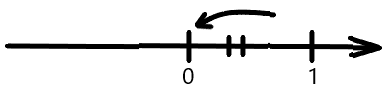
\includegraphics[scale=0.3]{22_0}

    \(x_n = -\frac{1}{n}\)
    \qquad 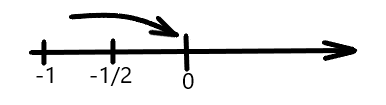
\includegraphics[scale=0.3]{22_1}

    \(x_n = \frac{(-1)^n}{n}\)
    
\end{enumerate}
    %RETHINK ALL "ARRAYS"
    \title{Числовые последовательности и их пределы}
    \author{Ученики 10-4 класса Оконешников Д.Д. и Паньков М.А. по лекции к.ф.-м.н. Протопоповой Т.В.}
    \date{от 21 апреля 2021 г.}
    \maketitle

    \section{Лекция №24}
    \subsection{Свойства бесконечно больших}

    \begin{enumerate}
        \item Если предел последовательности \( \lim_{n \rightarrow \infty }a_n = + \infty \)\( (+\infty + c) \), а \( \{b_n\} \) ограничена снизу, т.е. \( b_n \geq b\ \forall n \), тогда \(\lim_{n \rightarrow \infty}{(a_n + b_n)} = +\infty\)
       
        \item Если \( \lim_{n \rightarrow \infty }a_n = + \infty \)\( (+\infty + c) \), а \( \{b_n\} \) ограничена \( M: b_n \geq M > 0,\ \forall n \)
    \(\lim_{n \rightarrow \infty}{(a_n * b_n)} = +\infty\)

        \item Если \( \lim_{n \rightarrow \infty }a_n = +\infty \), а \( b_n \) ограничена, т.е. \( 0 < b_n < M (n \rightarrow \infty)\ \forall n \), то \[ (\frac{+\infty}{c > 0}) \lim_{n \rightarrow \infty}{\frac{a_n}{b_n}} = +\infty\]
    
        \item Если \(\lim_{n \rightarrow \infty}{a_n} = \infty\), а \(b_n\) ограничена; \(\abs{b_n} \leq M\  \forall n\), \[ (\frac{M}{\infty}) \lim_{n \rightarrow \infty }\frac{b_n}{a_n} = 0 \].
    \end{enumerate}

    \subsubsection{Неопределённости}

    \textbf{1)} \(\infty - \infty\)
    \\ \(2n - n = n \rightarrow +\infty\)
    \\ \(\lim_{n \rightarrow \infty}{\sqrt{n+1} - \sqrt{n}} = \lim_{n \rightarrow \infty}{\frac{n+1-n}{\sqrt{n+1}+\sqrt{n}}}\) = 0

    \textbf{2)} \( \frac{\infty}{\infty} \)

    \( n^2,\ n,\ 2n \)
    
    \( \frac{n^2}{n}  \) % TODO !!!!!!!!

    \textbf{3)} \(\infty * 0\)
    
    \subsection{Теорема Вейерштрасса}

    \textbf{Определение.}
    Числовая последовательность целых чисел называется стабилизирующейся к \(\xi\), если \( \exists\ n_0\ \forall n > n_0\  a_n = \xi: a_n \rightarrow \xi \)
    
    \textbf{Лемма 1.}
    Если \(\{a_n\}\) --- последовательность целых неотрицательных чисел, неубывающая и ограниченная сверху, т.е. \( a_n \leq N\ \forall n\), то \( \exists\ \xi: a_n \rightarrow \xi \) и \( \xi \leq M \).

    % IMAGE TODO!!!!
    % FOLLOWING TEXT RIGHT TO IMAGE
    хотя число членов последовательности \(\infty\), но между \(a_1\) (самый маленький член последовательности т.к. \( a_n \not\searrow \)) и \(M\) есть только конечное число целых чисел, \(\Rightarrow\) только конечно число значений \(a_n\)\\
    Обозначним наибольшее значение принимаемое \( a_n \), ч/з \( \xi \), т.е. \( \exists n_0: a_{n_0} = \xi \leq M \), тогда \( \forall n > n_0\ a_n = \xi \), т.к. \( a_n \downarrow \)
    
    \(\{a_n\}\) --- б.д.д. > 0
    
    \(a_1 = \alpha_{10},\alpha_{11}\alpha_{12}\alpha_{13}...\)\\
    \(a_2 = \alpha_{20},\alpha_{21}\alpha_{22}\alpha_{23}...\)\\
    \(a_3 = \alpha_{30},\alpha_{31}\alpha_{32}\alpha_{33}...\)\\
    ...\\
    \(a_n = \alpha_{n_0},\alpha_{n_1}\alpha_{n_2}\alpha_{n_3}...\)\\
    \(\downarrow a = \gamma_0,\gamma_1\gamma_2\gamma_3...\)

    \(\alpha_{n_0}\) --- целые неотр.\\
    \(\alpha_{n_j}\  j = 1, ...\) --- это \(\in \{0,\ 1,\ 2, \ ..., \ 9\}\)

    \textbf{Определение.} Будем говорить, что последовательность б.д.д. \( (>0) \{a_n\} \rightrightarrows \)\\
    \( a = \gamma_0,\gamma_1\gamma_2\gamma_3...\ (a_n \rightarrow a) \), если \(\forall k \ \alpha_{n_k} \rightrightarrows \gamma_k\)

    \textbf{Лемма 2.} Если \( \{a_n\} \) --- последовательность неотрицательных б.д.д. (*) является неубывающей и ограниченной (т.е. \( \exists M \) (б.д.д., не оканчивающася последовательностью 9-ок)): \( \forall\ n\ a_n \leq M) \), то \( \exists\ a \):
    
    1) \(a_n \rightrightarrows\ a\)  

    2) \(a_n \leq a \leq M\)

    \( \uparrow \) В табл. (*) cмотрим на первый столбец

    \( \alpha_{10} \)\\
    \( \alpha_{20} \)\\
    \( \alpha_{30} \)\\
    ...\\
    \( \alpha_{n0} \)

    Это последовательность неубывающих целых неотр. чисел и ограниченных сверху \(M\) по \textbf{Л1}\\
    \(\exists \) номер \(N_0\) \: \(\forall\ n > N_0\)\\
    \(\ \alpha_{n_0} \rightrightarrows\ \gamma_0\)
    
    \( \alpha_{10} \)\\
    \( \alpha_{20} \)\\
    \( \alpha_{30} \)\\
    ...\\
    \( \alpha_{N_00} = \gamma_0 \)\\
    \(\gamma_0\)\\
    \(\gamma_0\)

    Пусть \(n > N_1\), тогда смотрим на \(\{\alpha_{n1}\}\)

    \(\alpha_{n1}\) --- последовательность целых, неотр. чисел. Она ограничена 9-кой; неубывающая(т.к. \(a_n \not\searrow\) и 0-й столбец уже застабилиз.) \(\Rightarrow \ \exists\ N_1 \ \alpha_{n_1} \rightrightarrows\ \gamma_1 \ \forall n > N_1 \geq N_0\)

    Пусть \( n > N_1 \geq N_0 \) и смотрим \( \{ \alpha_{n2} \} \)
    
    \(\{\alpha_{n2}\}\) --- последовательность целых, неотр. чисел. Она ограничена 9-кой, неубывающей(т.к. \(a_n \not\searrow\) и 1-ый столбец уже застабилиз.) \(\Rightarrow \ \exists N_2 \ \: \ \forall n > N_2 \geq N_1 \geq N_0 \ \alpha_{n2} \rightrightarrows\ \gamma_2\) и т.д.

    в итоге \( \forall\ n > N_k \geq N_{k-1} \geq ... \geq N_0\quad \{ \alpha_{nk} \} \rightrightarrows\ \gamma_k \), то \( a_n \rightrightarrows\ a = \gamma_0,\gamma_1\gamma_2\gamma_3...\gamma_k... \)
    
    Из построения \(a_n \leq a \)
    \\ Осталось показать, что a \(\leq\) M

    Будем доказывать от противного: т.е. пусть \(a > M\), т.е. \(a_{(k)} = \gamma_0,\ \gamma_1,\ \gamma_2,\ ...,\ \gamma_k > M\)
    \\ \(a_k\) --- прибл. по недост. для a, но тогда \(a_n \ \: \ n > N_k\)
    \\ \(a_n = \alpha_{n0},\ \alpha_{n1},\ \alpha_{n2},\ ...,\ \alpha_{nk},\ \alpha_{nk+1},\ ... = \gamma_0,\ \gamma_1,\ ...,\ \gamma_k\alpha_{nk+1} > a_{(k)} > M\), противоречие с тем, что \(a_n \leq M \ \forall n \ \downarrow\)

    \subsubsection{Теорема Вейерштрасса}

    Если \(\{ x_n \} \) --- числовая последовательность неубывает и ограничена сверху, то она сходится.

    \(\uparrow\)
    \begin{enumerate}
        \item Пусть \( x_1 > 0 \Rightarrow \forall\ n\ x_n > 0 \) т.к. \( (x_n \not\searrow ) \).

        \item Любое \( x_n \in \mathbb{R} \) представлена в виде б.д.д.

        \item По \textbf{Л2}, такая (1) \( x_n \rightrightarrows a \)

        \item Покажем, что \(x_n \longrightarrow_{n \rightarrow \infty} a\)
    \\ Надо \(\forall \varepsilon > 0 \ \exists N \ \: \ \forall n > N\), \(\abs{x_n - a} < \varepsilon\)

    пусть \( n > N_k \), где \( N_k \) - номер, когда \(k\)-ый столбец в (*) застабилиз., тогда 
    \[ \abs{x_n - a} = \abs{\gamma_0,\gamma_1....\gamma_k\alpha_{nk+1}\alpha_{nk+2}... - \gamma_0,\gamma_1\gamma_2...\gamma_k\gamma{k+1}\gamma_{k+2}...} \]
    \[ = 0,\underbrace{0...0}_k\beta_{k+1}\beta_{k+2}... < 0,\underbrace{0...0}_{k-1}1 = \frac{1}{10^k} < \frac{1}{9k} < \varepsilon \]
    \[k > \frac{1}{9\varepsilon}\quad \varepsilon \rightarrow k \rightarrow N_k = N \downarrow \]
    \end{enumerate}

    \textbf{Замечание 1.} 
    Если \(x_1 < 0\), тогда рассм. \(y_1 = x_1 + c\ : \ y_1 > 0\), тогда по доказ. \( y_n = x_n + c \not\searrow \), ограничена сверху и \( y_1 > 0 \Rightarrow \) по доказ \(y_n \xrightarrow[n \rightarrow \infty]{}\ \Rightarrow ............. \)
    
    \textbf{Замечание 2.}
    Аналогично можно доказать, что, если \(\{x_n\} \not\nearrow\) и ограничена снизу, то она сх-ся.
    
    В общем случае:
    \\ Если последовательность монотонна и ограничена, то она сх-ся \(\downarrow\)
    
    \textbf{Пример.}

    \(a_{n+1} = \frac{a_n + 1}{2}\); \(a_1 = 2\), доказать, что \(\{a_n\}\) сх-ся и найти \(lim\).

    \(a_1 = 2;\ a_2 = \frac{1}{2}(2+1) = \frac{3}{2};\ a_3 = \frac{5}{4};\ a_4 = \frac{9}{8}\)
    \\ Предположение: \(\searrow\) и \(1 < a_n \leq 2\)

    \(a = \frac{a+1}{2} \\ 2a = a + 1 \\ a = 1\)

    I. Покажем, что \(1 < a_n \leq 2\)
    \ \ \ \ 1) База \(n = 1 \quad 1 < a_1 = 2 \leq 2\) верно

    \ \ \ \ 2) Пусть при \(n = k \quad 1 < a_k \leq 2\) выполнено

    \ \ \ \ 3) Надо при \(n = k + 1 \quad 1 < a_{k+1} \leq 2\)
    \\ \(1 = \frac{1}{2}(1+1) < \textrm{ (по ПИ) } a_{k+1} = \frac{a_k + 1}{2} = \frac{1}{2}(a_k + 1) \leq \frac{1}{2}(2 + 1) = \frac{3}{2} \leq 2\)
    \\ \(\Downarrow\) по ПМИ \(\forall n \ 1 < a_n \leq 2\)

    II. \( a_{n+1} - a_n \) = \( \frac{(a_n+1)}{2} - a_n = \frac{1-a_n}{2} (a_n > 1\) из опр \(<0) < 0 \Rightarrow a_{n+1} < a_n \forall\ n \in N \) т.е. \( a_n \) - убыв.

    III. Из I и II по Т. Вейерштрасса \( \exists\ lim_{n \rightarrow \infty}a_n \). Пусть \(lim_{n \rightarrow \infty } = a \Rightarrow a = \frac{a + 1}{2} \Rightarrow a = 1 \)


\title{Числовые последовательности и их пределы}
\author{Ученики 10-4 класса Оконешников Д.Д. и Паньков М.А. по лекции к.ф.-м.н. Протопоповой Т.В.}
\date{от 28 апреля 2021 г.}
\maketitle

\section{Лекция №25}

\(\lim_{n \rightarrow \infty}{(1 + \frac{1}{n})^n}\)
\\ \(1^{\infty}\)
\\ \( x_n \xrightarrow[n \rightarrow \infty ]{}\ ? \)

\subsection{Число e}
1) \( \{ x_n \} \) --- ограничена \\
2) \( \{ x_n \} \) --- монотонна \\
Из 1) и 2) \( \Rightarrow \) сходятся

\textbf{I монотонна и возрастает}

\((a+b)^n = \sum_{k=0}^n\ C^k_n \ a^{n-k}b^k=1*a^n+\sum_{k=1}^n\ C^k_n \ a^{n-k}b^k = a^n+\sum_{k=1}^n \frac{n!}{k!(n-k)!} a^{n-k}b^k = \)

\( = a^n + \sum_{k=1}^n \frac{n(n-1)(n-2)...(n-(k-1))}{k!} a^{n-k} b^k\)

\( x_n = 1 + \sum_{k=0}^n \frac{n(n-1)(n-2)...(n-(k-1))}{k!} \frac{1}{n^k} = 1 + \frac{1}{1!} \frac{n}{n} + \frac{1}{2!} \frac{n(n-1)}{n^2} + \frac{1}{3!} \frac{n(n-1)(n-2)}{n^3} + ... + \)

\( + \frac{1}{k!} \frac{n(n-1)...(n-(k-1))}{n^k} + ... + \frac{1}{n!} \frac{n(n-1)...(n-(n-1))}{n^n} = 1 + 1 + \frac{1}{2!} \frac{n-1}{n} + \frac{1}{3!} \frac{(n-1)(n-2)}{n^2} + ... + \frac{1}{k!} \frac{(n-1)(n-2)...(n-(k-1))}{n^{k-1}} + ... +\)

\(x_n = 1+1+\frac{1}{2!}(1-\frac{1}{n})+\frac{1}{3!}(1-\frac{1}{n})(1-\frac{2}{n})+...+\frac{1}{k!}(1-\frac{1}{n})(1-\frac{2}{n})...(1-\frac{k-1}{n}) + ... + \frac{1}{n!} (1 - \frac{1}{n})(1 - \frac{2}{n})(1 - \frac{n-1}{n})\)

\((a+b)^{n+1} = \sum_{k=0}^{n+1}\ C_{n+1}^k a^{n+1-k} b^k = a^{n+1} + \sum_{k=1}^{n+1} \frac{(n+1)n(n+1-2)...(n+1-(k-1))}{k!} a^{n+1-k} b^k\)

\(x_{n+1} = 1 + 1 + \frac{1}{2!}(1-\frac{1}{n+1}) + \frac{1}{3!}(1-\frac{1}{n+1})(1-\frac{2}{n+1})+...+\frac{1}{k!}(1-\frac{1}{n+1})(1-\frac{2}{n+1})...(1-\frac{k-1}{n+1})+...+\frac{1}{n!}(1-\frac{1}{n+1})(1-\frac{2}{n+1})...(1-\frac{n-1}{n+1}) + \underbrace{\frac{1}{(n+1)!}(1-\frac{1}{n+1})(1-\frac{2}{n+1})...(1-\frac{n}{n+1})}_{> 0} \Rightarrow TODO \)

\(\frac{1}{n} > \frac{1}{n+1}\)

\(-\frac{1}{n} < -\frac{1}{n+1}\)

\(0 < (1-\frac{1}{n}) < (1-\frac{1}{n+1})\ n > 1\) 
\\аналог: \\\(0 < 1-\frac{2}{n} < 1-\frac{2}{n+1} \Rightarrow (1-\frac{1}{n})(1-\frac{2}{n}) < (1 - \frac{1}{n+1})(1 - \frac{2}{n+1})\)
\\\(\forall n \ x_n < x_{n+1} \Rightarrow\) возрастает

\textbf{II ограничена}

\( 2 < x_n < 2 + \frac{1}{2!} + \frac{1}{3!} + \frac{1}{4!} + ... + \frac{1}{k!} + ... + \frac{1}{n!} \)

\( < \)

\( \frac{1}{1*2} = \frac{1}{2} \)

\( \frac{1}{2*3} < \frac{1}{2*2} = \frac{1}{2^2} \)

\( \frac{1}{3*4} < \frac{1}{2*2*2} = \frac{1}{2^3} \)

\(< 2 + \frac{1}{2} + \frac{1}{2^2} + \frac{1}{2^3} ... \frac{1}{2^{k+1}}+...+\frac{1}{2^{n-1}} = 2 + \frac{\frac{1}{2} - \frac{1}{2^n}}{1 - \frac{1}{2}} = 2 + \frac{\not\frac{1}{2}(1-\frac{1}{2^{n-1}})}{\not\frac{1}{2}} = 3 - \frac{1}{2^{n-1}} < 3\)

\( x_n \nearrow \)\\
\(\underbracket{2 < x_n < 3}_{\Downarrow} \)\\
по теореме Вейерштрасса:\\
\( \exists\ \lim_{n \rightarrow \infty} (1 + \frac{1}{n})^n = e \)
\\\(e \approx 2.718281828459045...\)

\(\lim_{n \rightarrow \infty}{(1 - \frac{1}{n})^n} = \lim_{n \rightarrow \infty}{(\frac{n-1}{n})^n} = \lim_{n \rightarrow \infty}{(\frac{1}{\frac{n-1+1}{n-1}})^n} = \lim_{n \rightarrow \infty}{(\frac{1}{(1 + \frac{1}{n-1})^{n-1}_{\rightarrow e}(1 + \frac{1}{n-1})_{\rightarrow 1}})^n} = e^{-1}\)

\subsection{Принцип вложенных промежутков}

\textbf{Теорема.} Пусть задана система замкнутых промежутков:\\
\(\sigma_n = [a_n; b_n]\ \forall n \in \mathbb{N}:\sigma_1 \supset \sigma_2 \supset ... \supset \sigma_n \supset \sigma_{n+1}\quad \forall\ n \in \mathbb{N}\)\\
\(\alpha_n = b_n - a_n \xrightarrow[n \rightarrow \infty]{} 0\)\\
Тогда \(\exists !\ c\ :\ c \subset \sigma_n\ \forall n \in \mathbb{N}\).

\(\uparrow\)
\begin{enumerate}
    \item \(a_1 \leq a_2 \leq a_3 \leq ... \leq a_n \leq ... \leq b_n \leq b_{n-1} \leq ... \leq b_1\)\\
\(\{ a_n \} \not\searrow\) и ограничена сверху любым \(b_n \forall n\ \Rightarrow\ b_n\) сх-ся по т. Вейерштрасса
\\\(\exists \lim_{n \rightarrow \infty}{a_n} = c_1 \quad c_1 \leq b_n \ \forall n\)
\\\(\{b_n\} \not\nearrow\) и ограничена любым \(a_n\ \forall n\) снизу
    \item \( c_1 = \lim_{n \rightarrow \infty} a_n = \lim_{n \rightarrow \infty} (a_n - b_n + n_n) = 0 + c_2 = c_2 \)\\
\( c_1 = c_2 = c \)\\
    \item уже в п.1 показали, что \(a_n \leq c \leq b_n\ \forall\ n\), т.е. \( c \in [a_n; b_n]\ \forall\ n \)
    %\(\uparrow\)
    \item Покажем, такое \( c\ \exists! \) от противного: пусть есть еще \( \overset{\sim}{c} \) --- общая точка всех промежутков \( \overset{\sim}{c} \neq c \), например, \( \overset{\sim}{c} < c \)

Тогда: \(\lim_{n \rightarrow \infty}{a_n} = c\ \Rightarrow\ \forall \varepsilon > 0 \ \exists N\ :\ \forall n > N, c - \varepsilon < a_n < c + \varepsilon\)

\(a_n > c - \varepsilon = \{\varepsilon = \frac{c-\overset{\sim}{c}}{2}\} = c - \frac{c - \overset{\sim}{c}}{2} = \frac{c + \overset{\sim}{c}}{2} > \frac{2c^{~}}{2} = \overset{\sim}{c}\)
\\\(\exists N\ :\ \forall n > N\ a_{n1} > \overset{\sim}{c}\) т.е. для \(n > N\ \overset{\sim}{c} \not\in [a_n; b_n]\) --- противоречие \(\downarrow\)
\end{enumerate}

\textbf{Замечание.}

1) \( [a_n; b_n]! \)\\
\( 1 - \frac{1}{n}; 1 \rightarrow (1, 1) = \emptyset \)
2) Верна для \(\mathbb{R}\), неверна для \(\mathbb{Q}\)

\subsection{Подпоследовательности}
\textbf{Определение.} Числовая последовательность \( \{b_k\} = \{a_{nk}\} \), где \( n_1 < n_2 < n_3 < ... < n_k < ... n_1,n_2,n_3 \in \mathbb{N} \)\\
последовательность натуральных чисел называется подпоследовательностью последовательности \( \{ a_n \} \).

\textbf{Пример.} \( a_n = \frac{1}{n} \quad 1;\frac{1}{2};\frac{1}{3};\frac{1}{4};\frac{1}{5};...;\frac{1}{100};... \)

\( b_k = \frac{1}{2k} \quad \frac{1}{2};\frac{1}{4};\frac{1}{6};...\frac{1}{100};...\)

\( b_k' = \frac{1}{2k+1} \quad \frac{1}{3};\frac{1}{5};\frac{1}{7};...\)

\( b_k'' = \frac{1}{k+3} \quad \frac{1}{4};\frac{1}{5};...\)

\( b_k''' = \frac{1}{3k} \quad ...\)

\(a_n = (-1)^n\)

\(b_k' = 1\)

\(b_k'' = -1\)

\textbf{Определение.} Если \(\exists\ \lim\) подпоследовательности \(b_k = a_{nk}\ \lim_{k \rightarrow \infty}{b_k} = b\), то b --- частичный предел последовательности \(\{a_n\}\).

\textbf{Пример.} \( a_n = (-1)^n \)\\
Частичные пределы: \( b_k' = 1,\ b_k'' = -1 \)
\\\(a_n = \sin{\frac{\pi n}{2}}\) % IMAGE HERE (CIRCLE)

\textbf{Теорема.} Если \(\{a_n\}\) --- сходится к а, то и все частичные пределы \(\{a_n\}\) тоже равны a.

\(\uparrow\ \lim_{n \rightarrow \infty}{a_n} = a\) % IMAGE 2 HERE

начиная с \(n > N\ a - \varepsilon < a_n < a + \varepsilon \ \forall \varepsilon\), но тогда \(\forall n_k > N \ a - \varepsilon < a_{nk} < a + \varepsilon \Rightarrow\) т.е. \(\lim_{k \rightarrow \infty}{a_{nk}} = a \ \downarrow\)

\textbf{Следствие.}

\( x_n = (-1)^n \)

Если \( \exists\ x_{nk} \textrm{ и } x_{nk}':\ \lim_{k \rightarrow \infty} x_{nk} \neq \lim_{k \rightarrow \infty} x_{nk}' \Rightarrow \not\exists\ \lim x_n \)

\textbf{Пример.} \\
\(a_n = \sin{\frac{\pi n}{2}}\)\\
\(a_{nk} = a_{2k} = \sin{\pi k} = 0\)\\
\(\sin{\frac{\pi n}{2}} = 1 \Rightarrow \frac{\not\pi n}{\not2} = \frac{\not\pi}{\not2} + 4\not\pi k \)\\
\( a_{4k + 1} = \sin{\frac{\pi(4k+1)}{2}} = \sin{2\pi k + \frac{\pi}{2}} = 1 \)
\end{document}
